% LaTeX template for MICS papers
% To Run:  pdflatex Sample.tex

\documentclass[12pt]{article}


\setlength{\oddsidemargin}{0in}
\setlength{\evensidemargin}{0in}
\setlength{\topmargin}{0in}
\setlength{\headheight}{0in}
\setlength{\headsep}{0in}
\setlength{\textwidth}{6in}
\setlength{\textheight}{9in}
\setlength{\parindent}{0in} 

\usepackage{graphicx} %For jpg figure inclusion
\usepackage{times} %For typeface
\usepackage{framed} % for \begin framed
 \usepackage{url}

\usepackage {tikz}
\pagestyle{plain}

\usetikzlibrary{positioning,fit,shapes.arrows,shadows}
\definecolor {processblue}{cmyk}{0.96,0,0,0}

\begin{document}




\title{Applying Convolutional Neural Networks to Per-pixel Orthoimagery Land Use Classification}

\author{
Jordan Goetze\\
Computer Science Department\\
North Dakota State University\\
Fargo, North Dakota. 58102\\
jordan.goetze@ndsu.edu
}
\date{} 

\maketitle
\thispagestyle{empty}

\section*{\centering Abstract}

Recently, the proliferation of Convolutional Neural Networks has spurred research in a wide range of fields such as image recognition, voice synthesis, and various other classification tasks. Over the last several years, the availability of satellite and other forms of orthoimagery has also increased due to the decreasing cost of capturing devices. The amount of annotated or labeled orthoimagery has not kept pace with the increased availability of imagery, largely due to the time complexity of labeling such data. Land cover usage classifications in particular would have many uses in agriculture. The United States Department of Agriculture's National Agricultural Statistics Service provides land cover usage data at a resolution of 30 meters, which compared with - for example - a 1 meter imagery resolution, leaves a large discrepancy between the quality of the raw image data and the labeling data. This research  uses these low quality labels along with high quality image data to train a model that attempts to perform per-pixel land use classification, in hopes to create a classifier that is able to predict several different classes of land use, up to or beyond the resolution accuracy of the much less adequate label data set. It is important to note however, that it is very difficult to evaluate if a model provides relatively better classifications based on the semantics of the input image, due to the low resolution of the image labels. This is because, an individual pixel in the image label will only represent one class per NxN meter area - in the case of our data set, a 30x30 meter area. That individual pixel may be a poor representation of features actually represented in the higher resolution image data. Thusly, we will attempt to demonstrate that, with enough data, a model may generate higher a resolution classification than the original imagery labels with a reasonable margin of error, and attempt to define a way to evaluate the effectiveness of the model despite the poor resolution of the image labels.


\newpage

\section{Introduction}

Per-pixel image classification, commonly referred to as image segmentation, has a wide range of applications such as scene labeling for autonomous driving systems or inferring relationships between objects in images. Land-use classification would fall under the realm of scene labeling, wherein instead of looking at an image of a scene, the model is given a birds-eye-view of a geographical feature. This style of imagery is commonly called orthoimagery. Orthoimagery is typically collected with either satellites or drones, and due to the decreasing cost of both apparatuses, the availability of orthoimagery has increased greatly over the last several years. 

One of many such projects to make orthoimagery available is the National Agricultural Imagery Program (NAIP) which is administered by The United States Department of Agriculture's Farm Service Agency. The NAIP data set imagery spans most of the continental United States of America. NAIP imagery is acquired at one-meter ground sample distance (GSD) and provides red, green, blue, and near infrared image layers. The United States Department of Agriculture's National Agricultural Statistics Service (NASS) also provides land-use classifications for the continental US, however, the resolution accuracy of these classifications limits their usefulness for agricultural surveying. As compared to the NAIP imagery resolution, one pixel of the NASS land-use classifications represents 50x50 pixels in a NAIP image, in other words a 50 square-meter area. Additionally, NASS classifications have many mislabeled pixels, visible by overlaying a NAIP image with a corresponding NASS classification image as seen in \textbf{Figure 1}. Additionally, as shown in \textbf{Figure 2}, regions with curved, or organic edges are often clipped. Finally, as in \textbf{Figure 3}, fine features are often not represented, or are poorly represented because they represent a minority of pixels in the mapped region.



\begin{center}
  \begin{framed}
    \centering{NAIP imagery overlaid with corresponding NASS land use classifications.}
  \end{framed}
  \begin{figure}[!htb]
    \minipage{0.32\textwidth}
      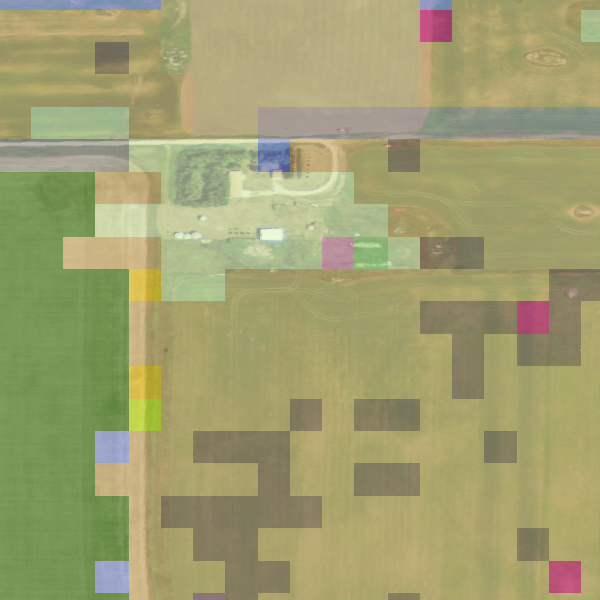
\includegraphics[width=\linewidth]{images/poor_labels_1.png}
      \caption{Mislabeled pixels.}
    \endminipage\hfill
    \minipage{0.32\textwidth}
      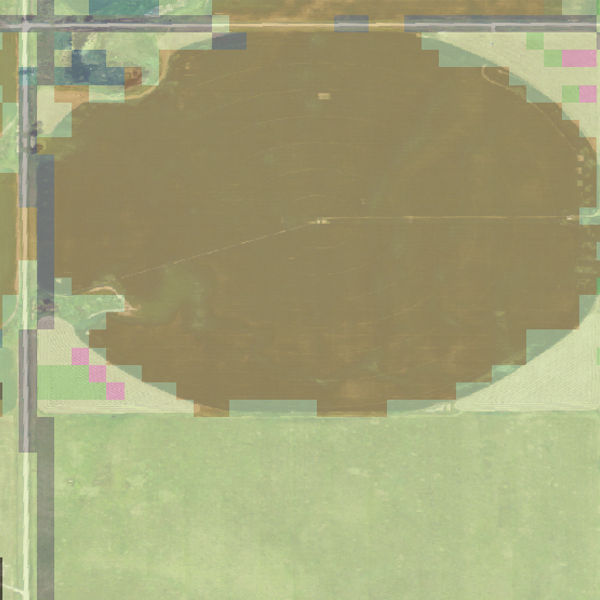
\includegraphics[width=\linewidth]{images/poor_labels_2.png}
      \caption{Clipped organic features.}
    \endminipage\hfill
    \minipage{0.32\textwidth}
      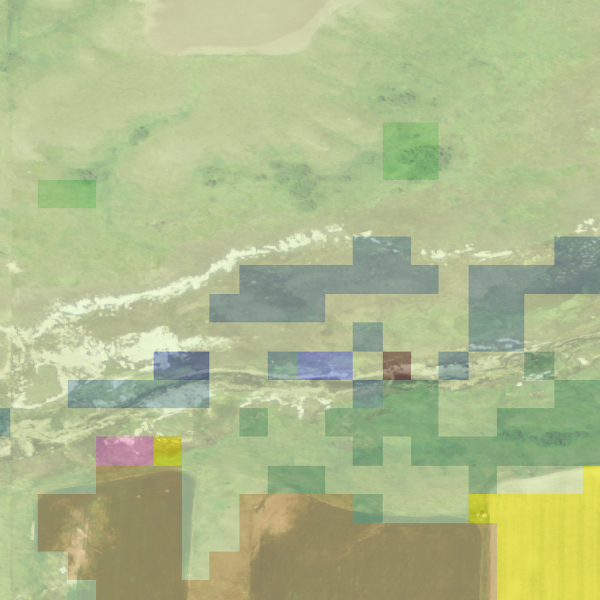
\includegraphics[width=\linewidth]{images/poor_labels_3.png}
      \caption{Fine features poorly represented.}   
    \endminipage 
  \end{figure}
\end{center}

\newpage

More accurate land-use classifications could be used for many tasks such as tracking crop yields by year, tracking changes in land use(crop rotations, new crops), tracking changes in forestry, and tracking changes in water sources such as rivers and lakes. Additionally, with a model able to generate accurate classifications, up to date classification data may be generated by processing new orthoimagery with the model. Unfortunately, successful image segmentation is a challenging problem.

\section{Related Work/Literature Review}

Much of previous orthoimagery segmentation and classification research has been focused on identifying roads and buildings, for use with mapping technologies such as Google Maps or Open Street Map. There seems to be very little research into the problem of generating classified segmentation for use with other applications such as natural resource surveying. Because per-pixel classifications of orthoimagery fall under the realm of scene recognition, we researched viable approaches to scene recognition. One of the notable works on scene recognition was SegNet. The SegNet publications outline a deep convolution encoder-decoder network which when applied to the CamVid data set produced good representations of features in the data set with relatively light computational requirements. The CamVid data set consists of ten minutes of high quality video imagery with corresponding semantically labeled images captured from a driving automobile. When applied to the CamVid data set, SegNet is able to produce high accuracy labels in real time. When searching for a staring point to begin with orthoimagery classification, it seemed worth while to see if the usefulness of SegNet was transferable to a new realm of sudy. The low computational requirements and the speed of the network were also attractive to minimise the upfront costs of hardware needed for training and testing a model.

SegNet's architecture\cite{SegNet} consists of several corresponding encoder-decoder layers. Each encoder layer consists of a convolutional operation, followed by a batch normalization operation, followed by a Rectified Linear Units (RELU) operation, followed by a max-pooling operation. It is important to note that the max-pooling indices are saved for later use. Each decoder layer consists of an upsampling operation, a convolution operation, a batch normalization operation, and a RELU operation. A softmax classification layer is placed at the end of the network to compute the probabilities of classes. For the upsampling operation, the max-pooling indices from the encoder layer are used as the indices to unpool the inputs. This upsampling method is one of the unique qualities of SegNet. Upsampling in this manner allows for rapid training of a model because the decoder does not need to learn how to upsample the down-sampled filter windows of the previous layer. Effectively allowing us to produce per-pixel classifications at the same resolution as the input image.


\newpage

\begin{figure}[!htb]
  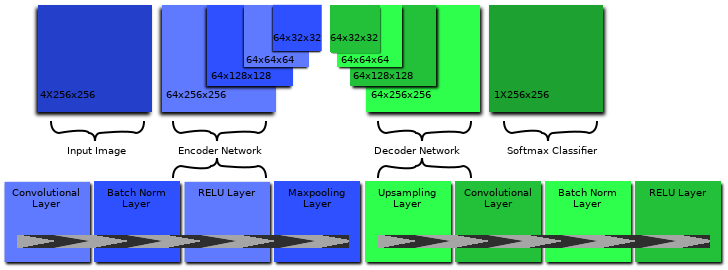
\includegraphics[width=\linewidth]{images/network.png}
  \caption{SegNet architecture. The encoder network consists of four sets of encoder layers of decreasing resolution. The decoder network consists of four sets of decoder layers of increasing resolution. The bottom row depicts the architecture of one encoder layer and one decoder layer. For every encoder layer, there is a matching decoder layer.}
\end{figure}
In more detail, each encoder layer performs a convolutionl operation to produce a set of feature maps. The feature maps are then batch normalized and a RELU operation is applied. Finally, a max-pooling operation is applied to the feature maps to ``reduce translational variance over small spacial shifts within the input image''\cite{SegNet}. The indices of the max-pooled samples are saved for use with a corresponding decoder layer. In each decoder layer, the corresponding indices are used to preform indice unraveling as a means of upsampling the feature maps. The upsampled feature maps are then convolved upon, batch normalized, and a RELU operation is applied. The resulting feature maps are then fed to a softmax classifier and per-pixel label-wise probabilities are computed. 


\section{Data Set Preprocessing}
As described above, our data sets consist of raw images from the National Imagery Program (NAIP), and land-use classification data from the National Agricultural Statistics Service (NASS). NAIP imagery is acquired at one-meter ground sample distance (GSD) and provides red, green, blue, and near infrared image layers \cite{NAIP}. Images from the NAIP data set are available for download via the EarthExplorer tool hosted by the United States Geographical Services. EarthExplorer allows users to query various geographical datasets and interfaces with a bulk data download application. Once the image data is downloaded, the GDAL library (Geospacial Data Abstraction Library) tooling is used to generate a set of shapefiles which are then uploaded to the NASS CropScape land use classification tool. CropScape allows users to upload points of interest as shapefiles and fetch land-use classification data for a region contained by the shapefile. Once the land-use classification data is downloaded, the GeoTiff files containing the data must be resized to match the resolution of the NAIP imagery files. GDAL, using the gdalwarp command, is used for this purpose. Because GeoTiff files are georectified, resizing the classification images does not offset pixels in the image and we do not need to worry about pixels in the resized image being anti-aliased or smoothed in some way which might produce invalid data. A script then slices the NAIP image and the NASS classifications into 256x256 pixel swatches, and stores each channel of the NAIP image in its own greyscale PNG file. The near-infrared layer is converted to a Normalized Difference Vegetation Index (NDVI) scaled from 0 to 255 (more on this is covered in the Architecture section). Classification images from NASS contain 255 different possible labels. In order to simplify these labels we grouped labels into one of 5 groups: forestry, developed, field, water, or background which we use as our labels to predict. The breakdown of which NASS labels were grouped into each label can be seen in Figure 6. Each classification swatch is stored as a greyscale image. Images are stored in this manner to allow easy visualization of the images. Because the input image consists of four layers: red, green, blue, and NDVI - the NDVI layer is interpreted by image viewers as an opacity layer which would make manual inspection of swatches difficult. During training and testing, these sets of image swatches are loaded in batches and passed into the model.


\begin{figure}
  \begin{tabular}[]{|p{2cm}|p{12cm}|}
  \hline
  Forestry & Forest, Shrubland, Christmas Trees, Other Tree Crops, Deciduous Forest, Evergreen Forest, Mixed Forest, Woody Wetland \\ \hline
  Developed & Fallow/Idle Cropland, Developed, Developed Open Space, Developed Low Density, Developed Medium Density, Developed High Density, Grass/Pasture \\ \hline
  Field (abridged) & Corn, Cotton, Rice, Sorghum, Soybeans, Sunflower, Peanuts, Tobacco, Sweet Corn, Pop or Oat Corn, Mint, Barley, Durum Wheat, Spring Wheat, Winter Wheat, Other Small Grains, Double Crop Winter Wheat and Soybeans, Rye, Oats, Millet, Speltz, Canola, Flaxseed, Safflour, Rape Seed, Mustard, Alfalfa, Other/Non-hay Alfalfa, Camelina, Buckwheat, Sugarbeets, Dry Beans, Potatoes, Other Crops, Sugarcane, Sweet Potatoes, Misc. Vegitables \& Fruites \\ \hline
  Water & Water, Aquaculture, Open Water, Herbaceous Wetlands \\ \hline
  Background & A catch-all class for the other classes that are either not used or too poorly represented. \\ \hline
  \end{tabular}
  \caption{Model classes to NAIP class breakdwon. Note that not all NAIP classes are represented in our classification data as most of our classifications come from North Dakota.}
\end{figure}


\begin{figure}
 \centering{
  \begin{tabular}[]{|p{2cm}|p{2cm}|p{2cm}|p{2cm}|p{2cm}|}
    \hline
    Forestry & Developed & Field & Water & Background \\ \hline
    0.63\% & 4.84\% & 76.26\% & 16.05\% & 2.22\% \\ \hline
  \end{tabular}
  \caption{Break down of class representation by percentage.}
 }
\end{figure}



\section{Architecture}

For the most part, our model encompasses a vanilla implementation of SegNet. The original SegNet model takes 4-band images as input. The first three bands correspond to the conventional red, green, and blue layers. The fourth band is a depth map scaled between 0 and 255. The fourth band in the image of our model is a Normalized Difference Vegetation Index (NDVI)\cite{NDVI} scaled between 0 and 255. The NDVI layer of our images is computed using the red and near-infrared layers of our source images using the following formula:  
\begin{figure}[!htb]
  \centering{
    $ NDVI = \frac{NIR-RED}{NIR+RED} $
  }
\end{figure}

NDVI is useful for tasks where vegitation is involved, this is due to the way near-infrared light reflects differently off of vegetation and non-vegetation.

Another difference between our model and the original SegNet model, is varying convolutional kernel sizes. We are currently experimenting with using different convolutional kernel sizes. SegNet recommends a 7x7 convolutional kernel size. This seems to work well for the SegNet data set image size and its task, however such a large convolutional kernel reduces sensitivity to fine features and does not work as well in our much smaller images (smaller images means noticeably finer features than in the CamVid data set). We have two different variations of our model which use 5x5 kernels and 3x3 kernels. The 5x5 kernel allows for detection of finer features than SegNet's 7x7 kernel. The 3x3 kernel allows for detection of even finer features than the 5x5 kernel. We expected that because of the higher sensitivity of the 3x3 kernel, the predictions would be more noisy as the model may begin to pick up on some of the image noise. We are also investigating using kernel sizes that vary for each encode decoder layer. For example, the first two encoder-decoder pairs would use a kernel size of 3x3 and the second two encoder-decoder pairs would use a kernel size of 5x5.

\section{Training and Evaluation}
The model is trained on 90\% of the available image swatches (approximately 72,000 image swatches) in batches of 15 for 25 epochs. While training we save checkpoints every 100 steps. Post training we then select the checkpoint with the highest evaluation accuracy. The model is evaluated on 10\% of the available images (approximately 8,000 image swatches). Evaluating and training with k-fold cross validation is planned for the future.

\section{Analysis}

\begin{figure}
 \centering{
  \begin{tabular}[]{|l|l|}
    \hline
    3x3 Convolutional Kernel & 71.61\% \\ \hline
    5x5 Convolutional Kernel & 73.33\% \\ \hline  
  \end{tabular}
  \caption{Evaluation accuracy of model variants.}
 }
\end{figure}

As our model is still in relative infantsy, results are still rather disappointing. With accuracies close to but still less than 76\% (as seen in Figure 7), we can see that for the vast majority of images, the model assumes that all pixels are of the field class. From there, it is attempting to recognize patterns in the image, and often times it picks up on image features, but does not correctly classify the pixels. Some of this may be because the label images are very low quality. A comparison between the label images and the model predictions can be seen in Figure 8.

\begin{figure}[!htb]
  \centering{
    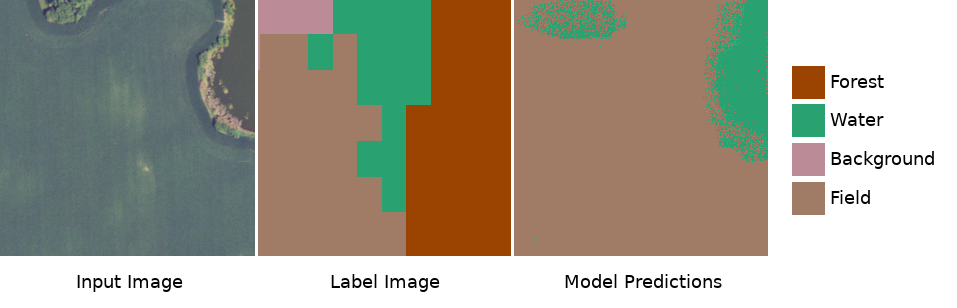
\includegraphics[width=\linewidth]{images/classification_better_than_labels_1.png}
    \caption{Model prediction producted by the 5x5 convolutional kernel model variation.}
  }
\end{figure}

\begin{figure}[!htb]
  \centering{
    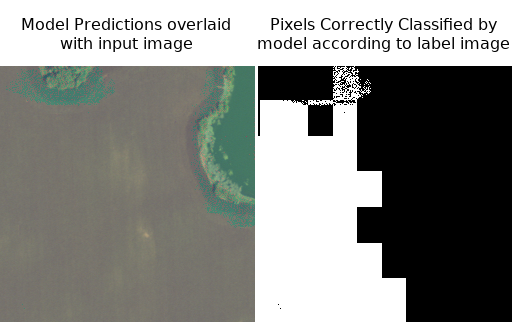
\includegraphics[width=300pt]{images/classification_better_than_labels_2.png}
    \caption{Model prediction evaluation corresponding to the predictions in Figure 8.}
  }
\end{figure}

 In Figure 8, the label image appears to be incorrectly labeled, as there appears to be no forest (trees or shrubland) in the input image. When we look at the comparison between the input image and the model prediction, we can see that the model prediction represents features in the input image much more closely than the label image. This comparison is more easily visible in Figure 9 where we have overlaid the input image with the model prediction. So while the model doesn't produce accurate labels when compared with the highly inaccurate label image, the model appears to visually provide a reasonable approximation (albeit noisy) of features in the image that can be differentiated by humans. This leaves us with the problem of figuring out how to correctly determine accuracy and error for the model. To further this point, the image on the right side of model 9 depicts the pixels that were classified correctly according to the label image. In this image white pixels represent a correct classification, and black pixels an incorrect classification. The blocky-ness of the borders between correctly and incorrectly labeled pixels (such as in the bottom half of the image) indicate that the model is struggling to cope with the difference in the resolution of the label images. As a result, the poorness of the image labels sometimes causes correct classifications to be counted as incorrect as in the right most image of Figure 10. The classification is a rounded, very organic feature. However, because of the low resolution of the image label, sharp corners appear in the classification accuracy image, resulting in a falsely lower reported accuracy for the image.

\begin{figure}[!htb]
  \centering{
    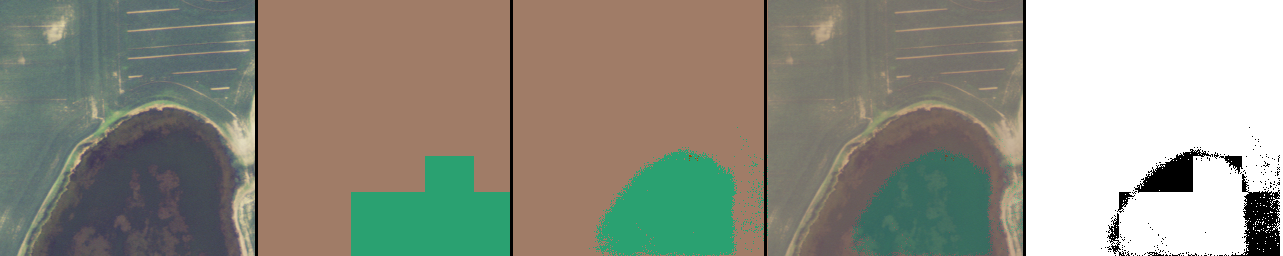
\includegraphics[width=\linewidth]{images/bad_image_labels.png}
    \caption{Model prediction produced by the 5x5 convolutional kernel model variation.}
  }
\end{figure}


\section{Future Work}

Though this research is an ongoing project, it is clear that significant changes need to be made to the model and process in order to achieve desirable results. We need to find some way of addressing the resolution discrepancy between the label images and the input images. Possible thoughts to this effect include attempting to find some way to take label images of two different resolutions, and somehow using them as a way of projecting a third higher resolution label image. 

Another idea is to define training and evaluation error differently. Training error would still be calculated based on the loss between the predictions and the NASS label images. Evaluation error would be based on a randomly sampled set of test images which we would manually label. We would then find some way of determining the error between the NASS label images and the manual label images and then remove that quantity of error from the prediction error. This approach works on the assumption that a human can accurately classify the image data, and that the amount of error between the NASS image labels and the manual image labels is somehow proportionate to the amount of error caused by the poor resolution of the label images as is visible in Figure 10.
We would also like to migrate to a more extensive training and evaluation setup where we would run the model with k-fold cross validation to get a more reliable measure of accuracy.

Finally, we would like to experiment more with the varying combinations of convolutional kernel filter widths to attempt to reach a balance between micro-features and macro-features, and ideally prevent the model from picking up on image noise while still retaining visibility of fine features. 

\section{Conclusion}

We have presented our modified SegNet model and have detailed our ongoing research into pixelwise image classification using orthoimagery. Though current results are nominal, we have plans to address the various concerns we believe are leading to this deficiency.
 
\bibliographystyle{plain}
\bibliography{mics_2017}

\end{document}
